\documentclass{beamer}
\usetheme{metropolis}
\setbeamercovered{transparent=25} 
\usepackage[utf8]{inputenc}
\usepackage{amsfonts,amsmath,oldgerm}
\usefonttheme[onlymath]{serif}
\usepackage{tikz}
\usepackage{xcolor}

\usepackage{subcaption}
\usepackage{float}
% \usepackage{floatrow}
% \usepackage{subfig}
% \usepackage{floatrow}

\usepackage[ruled]{algorithm2e}
\makeatletter
\newcommand{\RemoveAlgoNumber}{\renewcommand{\fnum@algocf}{\AlCapSty{\AlCapFnt\algorithmcfname}}}
\newcommand{\RevertAlgoNumber}{\algocf@resetfnum}
\makeatother

\usepackage{hyperref}
\hypersetup{
    colorlinks=true,
    linkcolor=blue,
    filecolor=magenta,      
    urlcolor=cyan,
    citecolor=blue,
    pdftitle={Overleaf Example},
    pdfpagemode=FullScreen,
    }
\usepackage[
backend=biber,
style=alphabetic,
sorting=ynt
]{biblatex}

\addbibresource{bibliography.bib}
% \usepackage{xargs}
% \usepackage[export]{adjustbox}

\newcommand{\greencheck}{\color{green}\checkmark}
\newcommand{\redcross}{\color{red}\times}
\newcommand{\tr}{\text{tr}}

\newcommand{\Tr}{\text{Tr}}

\newcommand{\mb}{\mathbf}

\newcommand{\bsy}{\boldsymbol}

\newcommand{\tb}{\textbf}

\newcommand{\ti}{\textit}

\newcommand{\btheta}{\boldsymbol{\theta}}

\newcommand{\brho}{\boldsymbol{\rho}}

\newcommand{\nmeasn}[1]{$n_{\text{meas}}=#1$}

\newcommand{\nitern}[1]{$n_{\text{iter}}=#1$}

\newcommand{\nburninn}[1]{$n_{\text{burnin}}=#1$}

\newcommand{\rhorankn}[1]{\text{rank}$(\rho)=#1$}

\newcommand{\nmeas}[0]{$n_{\text{meas}} $ }

\newcommand{\niter}[0]{$n_{\text{iter}} $ }

\newcommand{\nburnin}[0]{$n_{\text{burnin}} $ }

\newcommand{\rhorank}[0]{\text{rank}$(\rho) $ }

\newcommand{\semitransp}[2][35]{\textcolor{fg!#1}{#2}}

\usetheme{default}
\addtobeamertemplate{navigation symbols}{}{%
    \usebeamerfont{footline}%
    \usebeamercolor[fg]{footline}%
    \hspace{1em}%
    \insertframenumber/\inserttotalframenumber
}
\title{Master's thesis: Numerical comparison of MCMC methods for Quantum tomography}
\author[Mokeev]
{ Danila Mokeev\\{\small Supervisors: Estelle Massart, Andrew Thompson and Tameem Adel}}
\institute[EPL]{Ecole Polytechnique de Louvain}
\date{21st of June 2024}
\titlegraphic{%\includegraphics[width=2cm]{logopolito}\hspace*{4.75cm}~%
   
\includegraphics[width=4cm]{figures/logo_ucl.jpg}
}
\AtBeginSection[]
{
  \begin{frame}
    \frametitle{Table of Contents}
    \tableofcontents[currentsection]
  \end{frame}
}

\begin{document}

\frame{\titlepage}

\begin{frame}{Scope of this thesis}
    \tb{Topic}: Markov chain Monte Carlo (MCMC) methods in Quantum tomography\medbreak
    \tb{Research questions:} 
    \begin{enumerate}
        \item How do these methods perform in different experimental setups?
        \item Why do some methods perform better than others?
    \end{enumerate}
    \tb{Purpose:}
    \begin{itemize}
        \item Enable new directions of research
        \item Help researchers make an informed choice for their use case 
    \end{itemize}
\end{frame}
\begin{frame}{Thesis contributions}
    \begin{enumerate}
        \item Numerically compare 2 MCMC algorithms, the prob-estimator and the Projected Langevin algorithm
        \item Propose 2 new algorithms to understand the impact of the prior and the algorithm on the accuracy
    \end{enumerate}
\end{frame}

\begin{frame}
\frametitle{Table of Contents}
\tableofcontents
\end{frame}

\section{Brief introduction to Quantum tomography}
\begin{frame}{Motivation behind Quantum tomography}
    Quantum tomography is a process to reconstruct the quantum state of a system.\medbreak
    There are some challenges to consider: 
    \begin{itemize}
        \item Quantum systems are inherently probabilistic
        \item A measurement can only be made once
        \item We can only measure the position or momentum, but not both
    \end{itemize}
\end{frame}
\begin{frame}{Quantum tomography: a diagram}
    Quantum tomography allows to address the existing challenges\medbreak %provides a solution to this problem.\medbreak
    % Key steps:
    % \begin{enumerate}
    %     \item Replicate the initial state of the system multiple times
    %     \item Measure each clone once
    %     \item Calculate the empirical probabilities
    %     \item Estimate the quantum state with any appropriate method
    % \end{enumerate}
    \begin{figure}[H]
        %experiments/iterations_no_avg_sep_prob_pl_mhs_mhgs
            \centering
            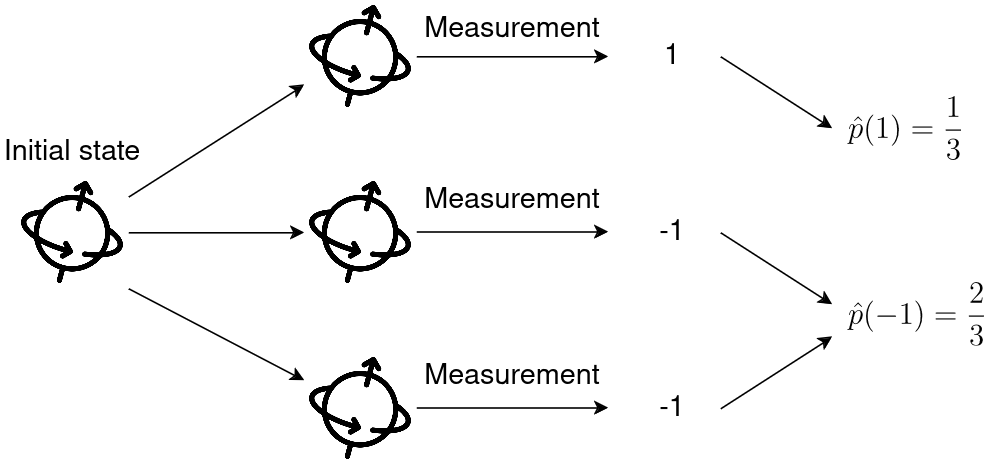
\includegraphics[width=\textwidth]{figures/diagram_qt_zoom_final.png}
            % 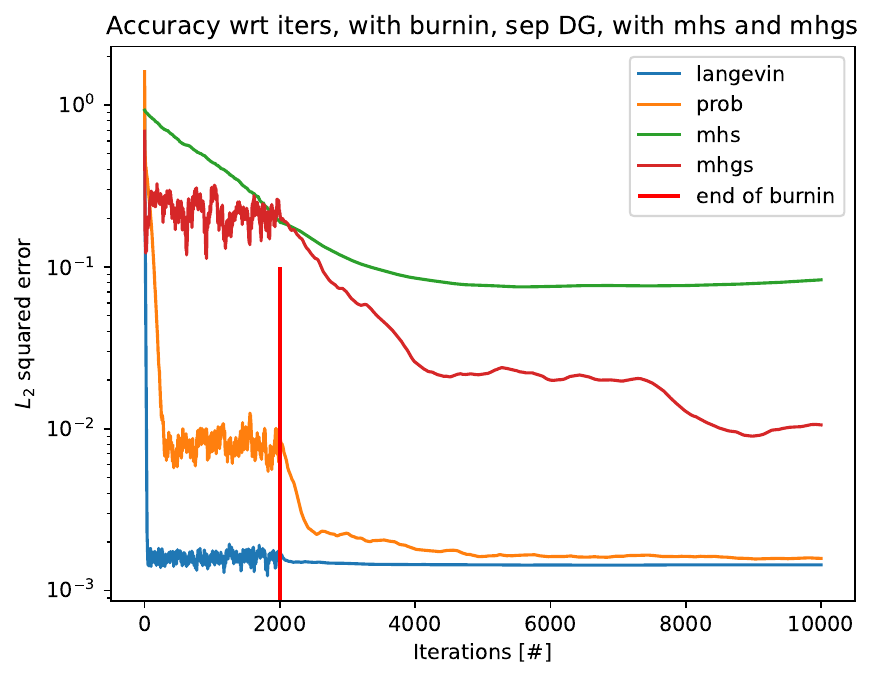
\includegraphics[width=0.7\textwidth]{figures/experiments/mhs_mhgs/iters_acc_comp_iters_no_avg_sep_prob_pl_mhs_mhgs-1.png}
        
            % \caption{Convergence plot with the prob-estimator, Projected Langevin, MHS, and MHGS with $n=3$ and separate qubit data generation}
        \end{figure}

\end{frame}

\begin{frame}{Quantum tomography: mathematical description (1)}
    The Born rule states that
    \begin{equation}
        p(m) = \tr(\rho P_m)
    \end{equation}
    with
    \begin{itemize}
        \item $p(m)$ the probability of occurence  of $m$
        \item $P_m$ the projector matrix associated to the eigenvalue $m$ of an \textit{observable} $O$
        \item $\rho$ the \textit{density matrix} representing the quantum state 
    \end{itemize}\medbreak
    The size of $\rho$ is  $2^n \times 2^n$ with $n$ the number of qubits.
\end{frame}
\begin{frame}{Quantum tomography: mathematical description (2)}
    If we flatten the matrices
    \begin{equation}
        A = \begin{bmatrix}
            P_{11} & P_{12} & P_{13} \cdots\\
            P_{21} & P_{22} & P_{23} \cdots\\
            \vdots & \vdots & \vdots \\
            P_{m1} & P_{m2} & P_{m3} \cdots
        \end{bmatrix}
        \quad\vec{\rho} = \begin{bmatrix}
            \rho_{11} \\
            \rho_{12} \\
            \rho_{13} \\
            \vdots
        \end{bmatrix}
    \end{equation}

    then we can estimate $\rho$ by solving the resulting system of equations 
    \begin{equation}
        A\vec{\rho} = \hat p
    \end{equation}
\end{frame}
\begin{frame}{Most common methods}
    \begin{itemize}
        \item Direct methods: \begin{equation}
            \hat \rho = (A^TA)^{-1}A^T \hat p
        \end{equation}
        \item Optimization-based methods: \begin{equation}
            \hat \rho = \text{argmin}_{\vec\rho} ||A \vec\rho - \hat p||
        \end{equation} 
        \item Pauli basis expansion:\begin{equation}
            \hat \rho = \sum_{b\in\{I,x,y,z\}^n} \rho_b \sigma_b
        \end{equation}
        \item Bayesian methods, and in particular MCMC methods
        \begin{equation}
        \hat \rho = \frac{1}{N}\sum_{i=1}^N \rho_i \quad \text{with } \rho_i \sim \pi(\rho|\mb D)
        \end{equation}
    \end{itemize}
\end{frame}
\begin{frame}{Existing methods: our focus in this thesis}
    \begin{itemize}
        % \semitransp{
        \item<0> Direct methods: \begin{equation}
            \hat \rho = (A^TA)^{-1}A^T \hat p
        \end{equation}
        \item<0> Optimization-based methods: \begin{equation}
            \hat \rho = \text{argmin}_{\vec\rho} ||A \vec\rho - \hat p||
        \end{equation} 
        \item<0> Pauli basis expansion:
        \begin{equation}
            \hat \rho = \sum_{b\in\{I,x,y,z\}^n} \rho_b \sigma_b
        \end{equation}
        % }
        \item<1> Bayesian methods, and in particular MCMC methods
        \begin{equation}
        \hat \rho = \frac{1}{N}\sum_{i=1}^N \rho_i \quad \text{with } \rho_i \sim \pi(\rho|\mb D)
        \end{equation}
    \end{itemize}
\end{frame}
\section{Markov chain Monte Carlo methods}
\begin{frame}{Bayesian framework}
    In the Bayesian framework:
    \begin{equation}
        \underbrace{\pi (\rho|\mb D)}_{\text{Posterior}} \propto \underbrace{\pi(\mb D|\rho)}_{\text{Likelihood}} \underbrace{\pi(\rho)}_{\text{Prior}}
    \end{equation}
    Recall that each term is a distribution!\medbreak
    In the context of Quantum tomography:
    \begin{itemize}
        \item Likelihood $\pi(\mb D|\rho) = \exp(-||A \vec\rho - \hat p||)$
        \item Prior $\pi(\rho)$ is method specific
        % \item Posterior $\pi (\rho|\mb D)$ corresponds to a distribution over density matrices $\rho$ after being fitted on the data
    \end{itemize}
\end{frame}
\begin{frame}{Markov chain Monte Carlo methods}
    \begin{itemize}
        \item Markov chain Monte Carlo (MCMC) methods \textit{sample} from $\pi (\rho|\mb D)$.
        \item They build a Markov chain of samples $\rho_1, \rho_2, \dots$ such that
        \begin{equation}
            f(x) =\pi (\rho|\mb D)
        \end{equation}
        with the equilibrium distribution $f(x)$ of the chain
        \item The density matrix is then calculated as
        \begin{align}
            \tilde \rho &= \mathbb{E}[\rho]= \int \rho \pi(\rho|\mb D) d\rho\\
            \Leftrightarrow \hat \rho &= \frac{1}{N}\sum_{i=1}^N \rho_i \quad \text{with } \rho_i \sim \pi(\rho|\mb D)
        \end{align}
        % \begin{equation}
            
        % \end{equation}
        % \begin{equation}
        %     \hat \rho = \frac{1}{N}\sum_{i=1}^N \rho_i \quad \text{with } \rho_i \sim \pi(\rho|\mb D)
        % \end{equation}
    \end{itemize}
\end{frame}

% \begin{frame}{The Metropolis-Hastings algorithm}
%     % \begin{itemize}
%     %     \item One of the most common MCMC algorithms
%     % \end{itemize}
%     \begin{algorithm}[H]\label{code:prob}

%         \DontPrintSemicolon
    
%         % \SetKwInOut{Input}{Input}
    
%         % \SetKwInOut{Output}{Output}
    
    
%         % %\underline{Prob-estimator}\;
    
%         % \Input{$d = 2^n, \lambda \in \mathbb{R}, \alpha \in \mathbb{R}, T \in \mathbb{N}, V^{(0)} \in \mathbb{C}^{d \times d}, Y^{(0)} \in \mathbb{C}^{d\times 1}$}
    
%         % \Output{$\hat \rho \in \mathbb{C}^{d\times d}$}
    
%         % $\hat \rho \gets \mb 0$\;
    
%         % $\gamma^{(0)} \in \mathbb{R}^{d\times1} \gets Y^{(0)} /(\sum_{i=1}^d Y_i^{(0)})$\;
    
%         \For{$t\gets 1:T$}{
%             \begin{enumerate}
%                 \item Generate a candidate $\rho^* \sim \overbrace{q(\rho|\rho^{(t-1)})}^{\text{proposal}}$
%                 \item Set $\rho^ {(t)} = \begin{cases}
%                     \rho^{*} \hspace{1.08cm} \text{with prob. } \alpha(\rho^*, \rho^{(t-1)})\\
%                     \rho^{(t-1)} \hspace{0.5cm} \text{with prob. } 1-\alpha(\rho^*, \rho^{(t-1)})
%                 \end{cases}$
%             \end{enumerate}
%             with \begin{equation}
%                 \underbrace{\alpha(\rho^*, \rho^{(t-1)})}_{\text{acceptance ratio}} = \frac{\pi(\rho^*|\mb D) q( \rho^{(t-1)}|\rho^*)}{\pi(\rho^{(t-1)}|\mb D) q( \rho^{*}|\rho^{(t-1)})}
%             \end{equation}
%         }
%         \caption{Metropolis-Hastings algorithm}

%     \end{algorithm}

% \end{frame}

\begin{frame}{An example: Metropolis-Hastings algorithm}
    \href{run:./mcmc.gif}{mcmc.gif}

\end{frame}

\begin{frame}{Advantages of MCMC algorithms}
    Why are we interested in MCMC methods?
    \begin{itemize}
        \item Prior $\pi(\rho)$: additional information about the density matrix - low-rank for example
        \item Uncertainty quantification: working with distributions instead of point estimates
    \end{itemize} 
\end{frame}
\section{Main algorithms}
\begin{frame}{Prob-estimator: prior}
    % Introduced in \cite{MA17}, it combines Metropolis-within-Gibbs sampling with a low-rank prior.
    \begin{itemize}
        \item Sum of rank-1 matrices: \[\rho = \sum_{i=1}^{d} \gamma_i V_i {V_i}^\dagger\]
        \item The prior $\pi_1(\gamma_1 \dots \gamma_d)$ is a Dirichlet distribution. A typical draw leads to a sparse vector.
        \begin{equation*}
            \gamma = \begin{bmatrix}
                0 & \cdots & 1 & \cdots & 0
            \end{bmatrix}
        \end{equation*}
        \item The prior $\pi_2(V_i)$ is a unit sphere distribution
        \begin{equation*}
            ||V_i|| = 1
        \end{equation*}
    \end{itemize}
\end{frame}

\begin{frame}{Prob-estimator: algorithm}
    % Mix between Metropolis-Hastings and Gibbs sampling\medbreak
    % \begin{example}{this is a block}
    %     \begin{quote}
    %         Notice
    %     \end{quote}
    % \end{example}
\begin{algorithm}[H]
    \RemoveAlgoNumber

    \DontPrintSemicolon
    
    \For{$t\gets 1:T$}{
        \alert<1>{}
    \pause
    % \alert<1>{
    %     \For{$i\gets 1:d$}{
    %         \pause
    %         \alert<2>{
    %     \begin{enumerate}
    %         \item Sample $ \gamma_i^*$ from $\pi_1(\gamma_i)$
    %         \item Update $\gamma^{(t)}$ with {accept/reject step}
    %     \end{enumerate}
    %         }\pause

    %     }} 
    \alert<2>{\tcp*[l]{Iterate over each dimension $i$}}\pause
            \For{$i\gets 1:d$}{

            \begin{enumerate}
                \alert<3>{\item Sample $ \gamma_i^*$ from $\pi_1(\gamma_i)$}\pause % \alert<2>{\tcp*[l]{Sample from the prior}}\pause
                \alert<4>{\item Update $\gamma^{(t)}$ with {accept/reject step}}\pause
            \end{enumerate}

            }
            \alert<5>{
            \For{$i\gets 1:d$}{
                \begin{enumerate}
                    \item Sample $V_i^*$ from $\pi_2(V_i)$
                    \item Update $V^{(t)}$ with an accept/reject step
                \end{enumerate}
        }}
    }

    \caption*{Prob-estimator algorithm}

\end{algorithm}
% Observe that:
% \begin{itemize}
%     \item There \textit{is} an accept/reject step
%     \item We iterate over each dimension for each iteration $t$
% \end{itemize}
\end{frame}
\begin{frame}{Projected Langevin: prior}
    % Introduced in \cite{ACMT2024}, it combines the Unadjusted Langevin algorithm with a \textit{different} low-rank prior.
    
    \begin{itemize}
        \item Burer-Monteiro factorization: $\rho = YY^\dagger$, with rank$(Y)=r$ 
        \item Low-rank prior: spectral scaled Student-t distribution
        % \begin{equation}
        %     \pi(Y) = C_\theta \det(\theta^2I_d + YY^\dagger)^{-(2d+r+2)/2}
        % \end{equation}
        \begin{equation}
            \pi(Y) = \prod_{j=1}^r (\theta^2 + \smash{\underbrace{s_j(Y)^2}_{j\text{th eigenvalue of } Y}})^{-(2d+r+2)/2}
        \end{equation}
        \item Promotes sparsity among the eigenvalues leading to a low rank
        \item Very similar to the Student-t distribution
        % \begin{itemize}
  
        % \end{itemize}
    \end{itemize} 
\end{frame}

\begin{frame}{Projected Langevin: algorithm}

    \begin{algorithm}[H]
        \RemoveAlgoNumber
        \DontPrintSemicolon
    
        \For{$t\gets 1:T$}{
            % \begin{equation}
            \begin{enumerate}
                \alert<1>{
                \item Sample $\tilde w^{(t)} \sim N(\mb 0, \mb I)$}\pause
                \alert<2>{
                \item $\tilde Y^{(t)} \gets \tilde Y^{(t-1)} - \eta^{(t)} \underbrace{\nabla \pi(\tilde Y^{(t-1)}| \mb D)}_{\text{\tb {gradient} }} + \cfrac{\sqrt{2\eta^{(t)}}}{\beta} \tilde w^{(t)}$}\pause
        \end{enumerate}
        }
    
        \caption*{Projected Langevin algorithm}
    
    \end{algorithm}
    The gradient allows us to explore the regions of high density faster.
\end{frame}
\section{Experiments and results}


\begin{frame}{Convergence plot}
    
\begin{figure}[H]
    %experiments/iterations_no_avg_sep_prob_pl_mhs_mhgs
        \centering
        \includegraphics[width=0.7\textwidth]{figures/experiments/baseline/iters_acc_comp_iters_no_avg-1.png}
        % 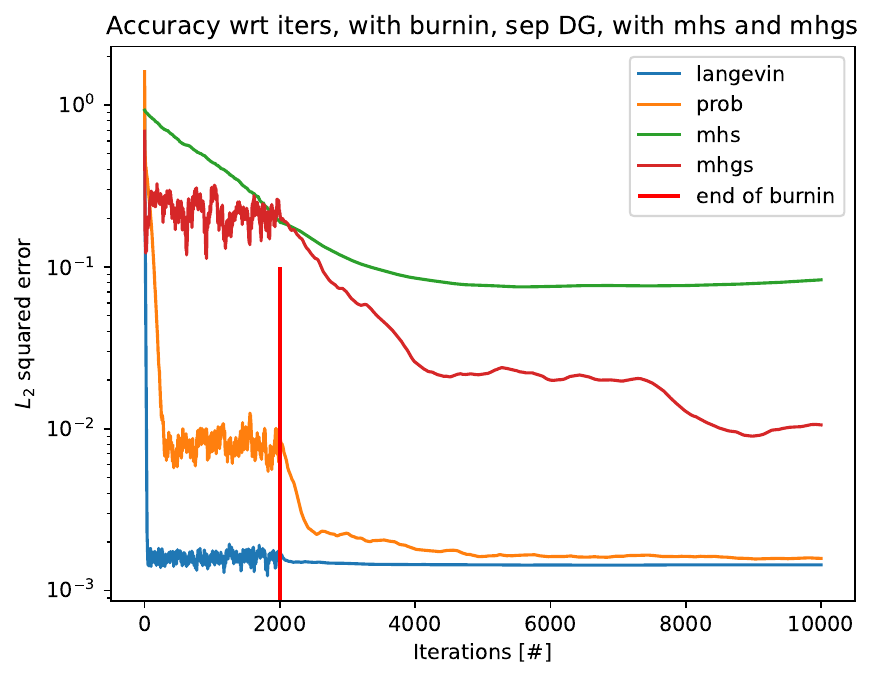
\includegraphics[width=0.7\textwidth]{figures/experiments/mhs_mhgs/iters_acc_comp_iters_no_avg_sep_prob_pl_mhs_mhgs-1.png}
    
        % \caption{Convergence plot with the prob-estimator, Projected Langevin, MHS, and MHGS with $n=3$ and separate qubit data generation}
        % \caption{$n=3$}
\end{figure}
$\Longrightarrow$ Projected Langevin converges faster for $n=3$ qubits
\end{frame}

\begin{frame}{Convergence speed for $n=4,5$}
    Reminder: a larger $n$ means a larger density matrix
    \begin{figure}[ht]

        \centering
    
        % \begin{subfigure}[t]{0.3\textwidth}
    
        %     % experiments/iterations_no_avg_rank1
    
        %     \centering
    
        %     \includegraphics[width=\textwidth]{figures/experiments/baseline/diff_n_qubits/iters_acc_comp_iters_no_avg-1.png}
    
        %     \caption{$n=3$}
        
        % \end{subfigure}
        
        \begin{subfigure}[b]{0.49\textwidth}
    
            % experiments/iterations_no_avg_n4
    
            \centering
    
            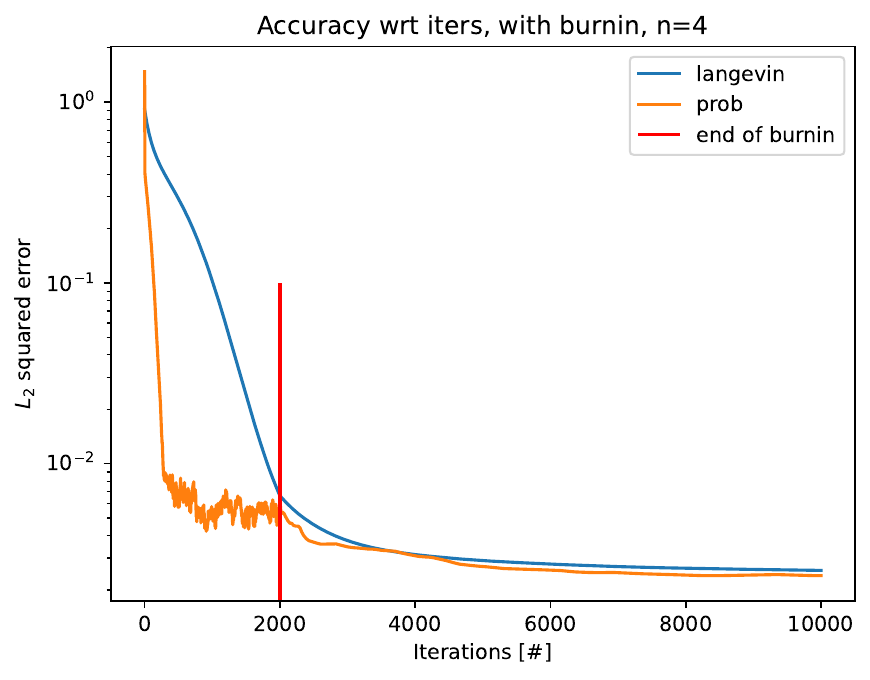
\includegraphics[width=\textwidth]{figures/experiments/baseline/diff_n_qubits/iters_acc_comp_iters_no_avg_n4-1.png}
    
            \caption{$n=4$}
        
        \end{subfigure}
        \hfill
        \begin{subfigure}[b]{0.49\textwidth}
    
            % experiments/iterations_no_avg_n5
    
            \centering
            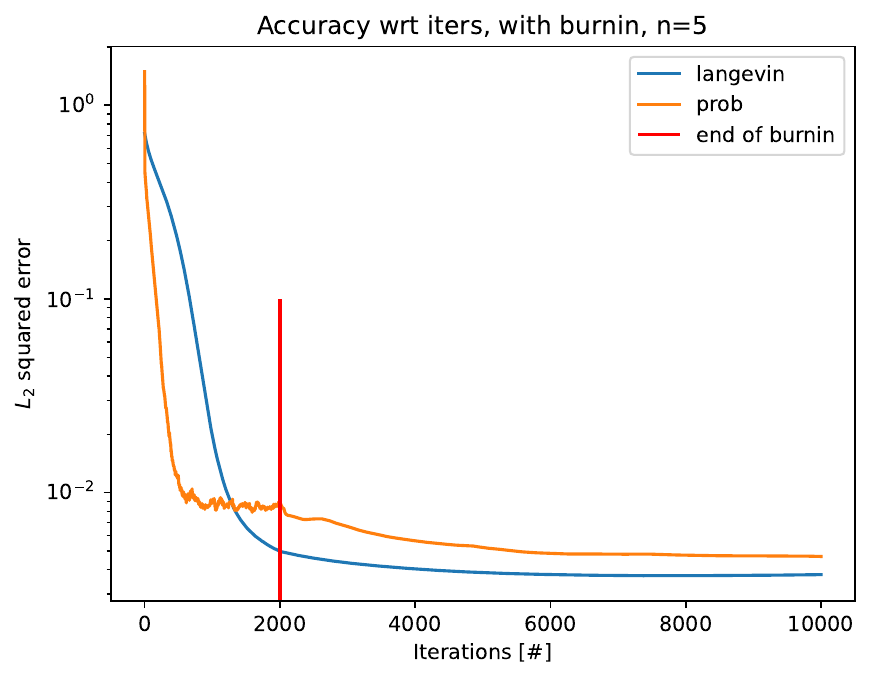
\includegraphics[width=\linewidth]{figures/experiments/baseline/diff_n_qubits/iters_acc_comp_iters_no_avg_n5-1.png}
            \caption{$n=5$}
        \end{subfigure}
   
            % \hspace*{\fill}
    \end{figure}
    $\Longrightarrow$ Projected Langevin converges slower than previously
\end{frame}
    
\begin{frame}{Computation time for $n=3$}
    
    \begin{figure}[H]
        \centering
    
        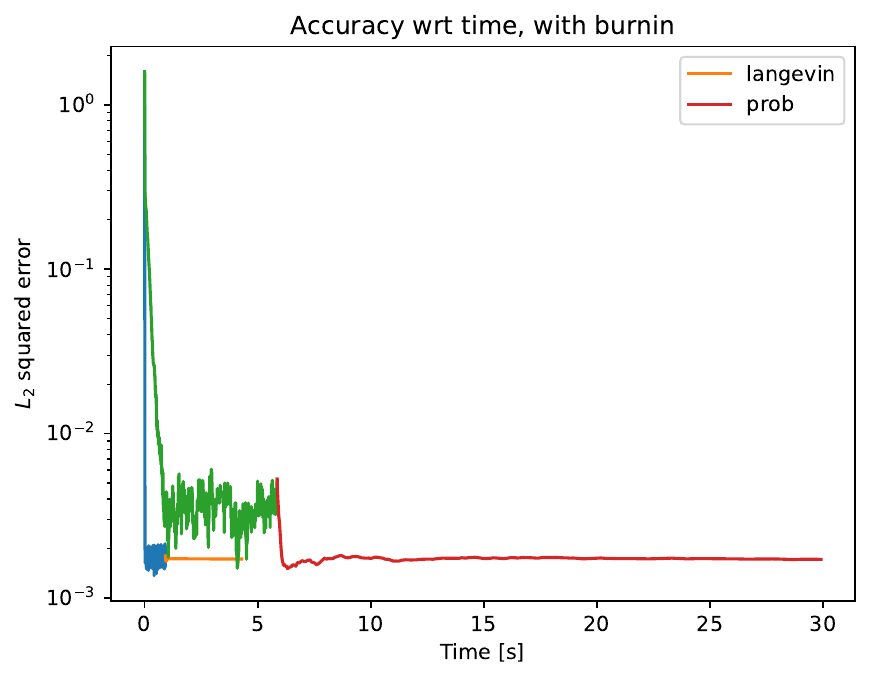
\includegraphics[width=0.7\textwidth]{figures/experiments/baseline/diff_n_qubits/iters_acc_comp_time_no_avg-1.png}

        % \caption*{$n=3$}

        % \label{fig:conv-plot-diff-n-3-sub}
    \end{figure}
    $\Longrightarrow$ For $n=3$, Projected Langevin takes much less time
\end{frame}

\begin{frame}{Computation time for $n=4,5$}
    
    \begin{figure}[H]

        \centering
    
        \begin{subfigure}[b]{0.49\textwidth}
    
            % experiments/iterations_no_avg_n4
    
            \centering
    
            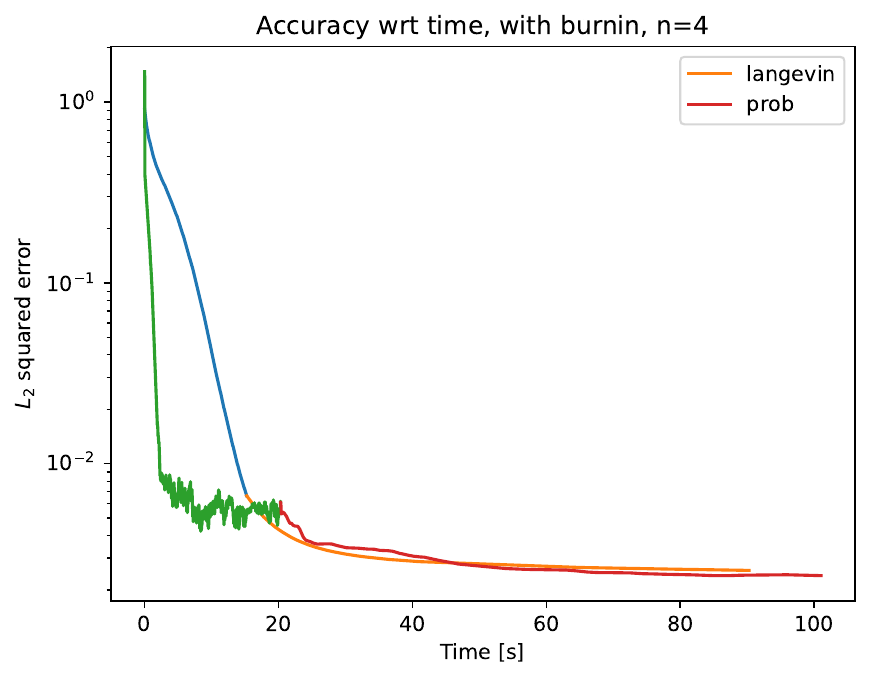
\includegraphics[width=\textwidth]{figures/experiments/baseline/diff_n_qubits/iters_acc_comp_time_no_avg_n4-1.png}
    
            \caption{$n=4$}
    
            \label{fig:conv-plot-diff-n-4-sub}
    
        \end{subfigure}
        \hfill
        \begin{subfigure}[b]{0.49\textwidth}
    
            % experiments/iterations_no_avg_n5
    
            
            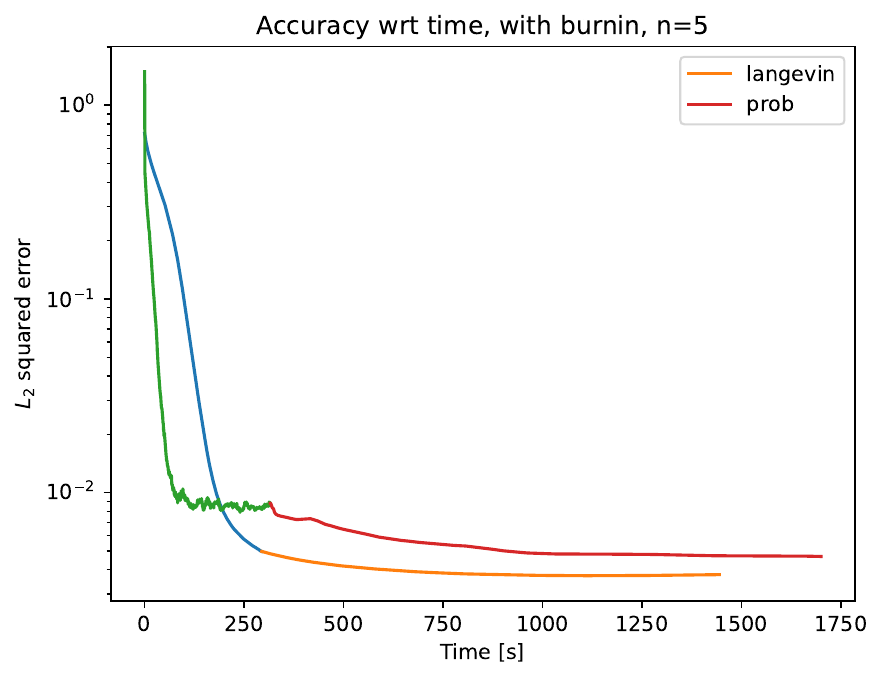
\includegraphics[width=\linewidth]{figures/experiments/baseline/diff_n_qubits/iters_acc_comp_time_no_avg_n5-1.png}
            \subcaption{$n=5$}
        \end{subfigure}
        \label{fig:conv-plot-diff-n}
    \end{figure}
    $\Longrightarrow$ When $n$ increases, Projected Langevin becomes as slow as the prob-estimator due to the gradient cost.

\end{frame}

\begin{frame}{Introducing 2 new methods}
    % Not happy about the slide
    What makes Projected Langevin perform better ?\medbreak
    To answer this question, we introduce 2 new algorithms:
    \begin{enumerate} 
    \item Metropolis-Hastings with Student-t prior (MHS)
    \item Metropolis-Hastings with Gibbs with Student-t prior (MHGS)
    \end{enumerate}
    They combine:
    \begin{itemize}
        \item The algorithm from the prob-estimator
        \item The prior from the Projected Langevin algorithm
    \end{itemize}
\end{frame}

\begin{frame}{Convergence comparison}
    \begin{figure}[H]
        %experiments/iterations_no_avg_sep_prob_pl_mhs_mhgs
            \centering
            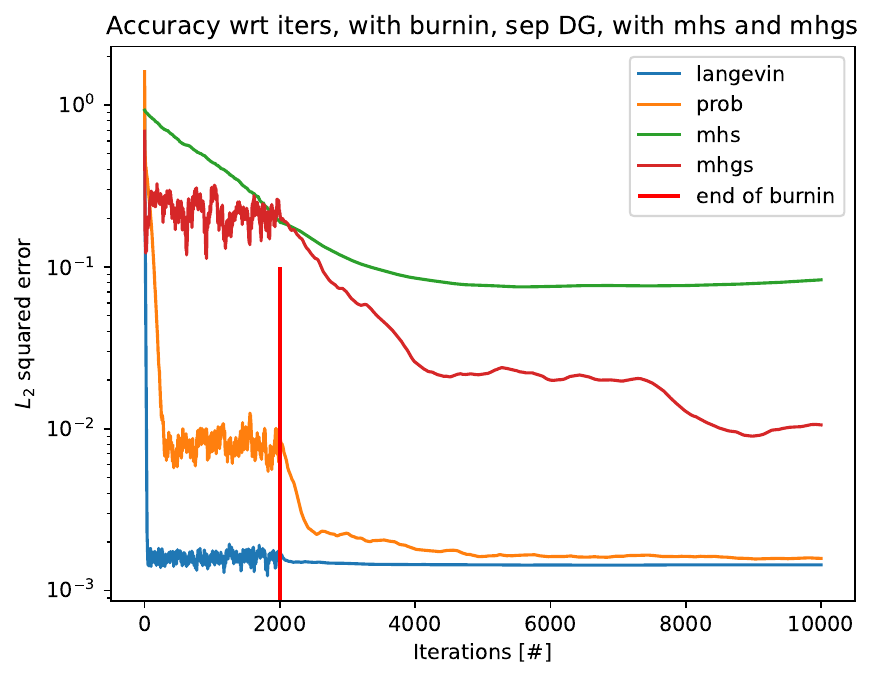
\includegraphics[width=0.7\textwidth]{figures/experiments/mhs_mhgs/iters_acc_comp_iters_no_avg_sep_prob_pl_mhs_mhgs-1.png}
            % 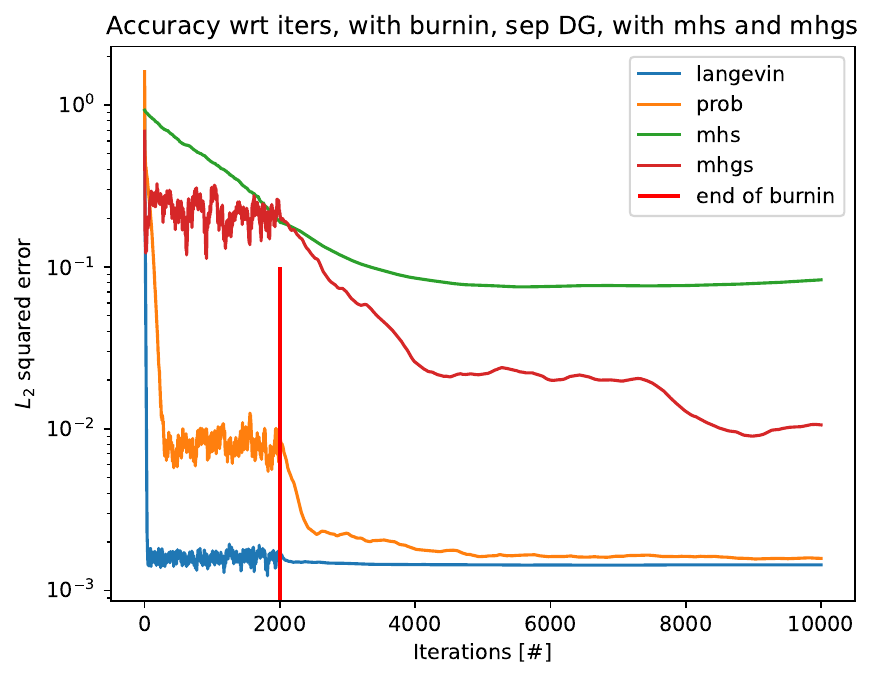
\includegraphics[width=0.7\textwidth]{figures/experiments/mhs_mhgs/iters_acc_comp_iters_no_avg_sep_prob_pl_mhs_mhgs-1.png}
        
            % \caption{Convergence plot with the prob-estimator, Projected Langevin, MHS, and MHGS with $n=3$ and separate qubit data generation}
        \end{figure}
        $\Longrightarrow$ The prior itself is not a solution, and must be paired with the right algorithm to be fast and accurate
\end{frame}

\begin{frame}{Impact of the number of shots}
    Shot: measurement we perform on a clone of the state
    \begin{figure}[H]

        \centering
        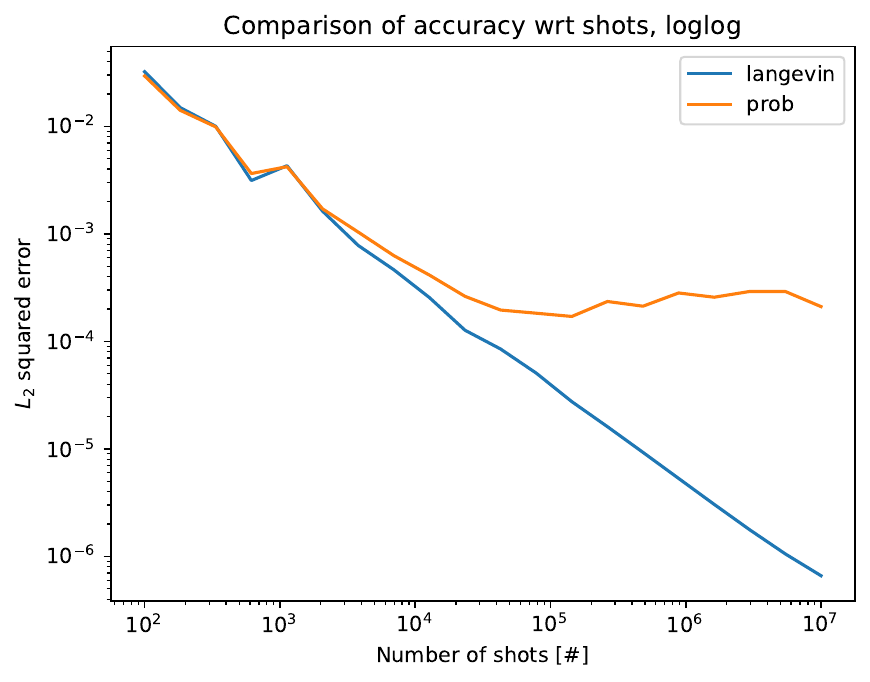
\includegraphics[width=0.7\textwidth]{figures/experiments/shots/shots_acc_comp_shots_exp_loglog-1.png}
        % \begin{subfigure}[b]{0.49\textwidth}
    
        %     % experiments/shots
    
        %     \centering
    
        %     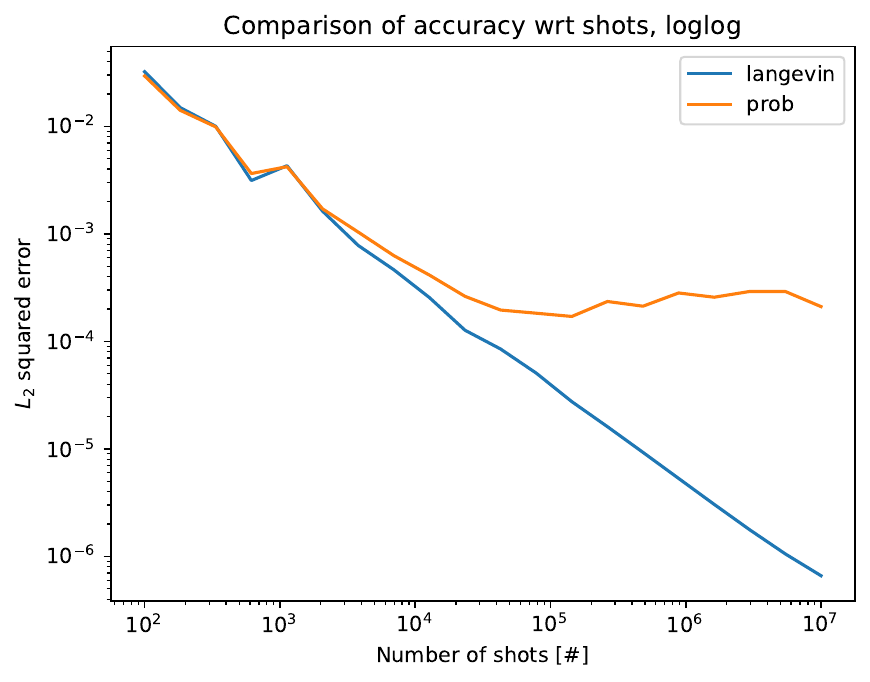
\includegraphics[width=\textwidth]{figures/experiments/shots/shots_acc_comp_shots_exp_loglog-1.png}
    
        %     \caption{Mixed qubit}
    
        %     \label{fig:shots-comp-mixed-sub}
    
        % \end{subfigure}
        % \hfill
        % \begin{subfigure}[b]{0.49\textwidth}
    
        %     % experiments/shots_sep
    
        %     \centering
    
        %     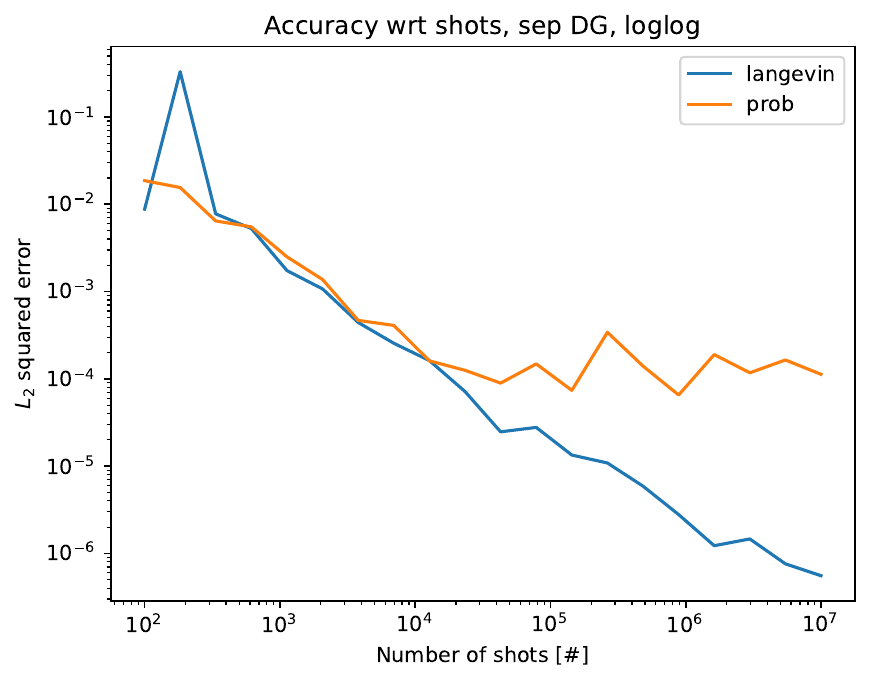
\includegraphics[width=\textwidth]{figures/experiments/shots/shots_acc_comp_shots_exp_sep_loglog-1.png}
    
        %     \caption{Separate qubit}
    
        %     \label{fig:shots-comp-sep-sub}
    
        % \end{subfigure}
        
        % \label{fig:shots-comp}
    
    \end{figure}
    $\Longrightarrow$ The prob-estimator does not scale!
\end{frame}

\begin{frame}{Impact of knowing the rank of $\rho$}
    Reminder: for Projected Langevin, $\rho = YY^\dagger$, with rank$(Y)=r$ 
    \begin{figure}[H]

        \centering
    
        \begin{subfigure}[b]{0.49\textwidth}
    
            % experiments/rank_known
    
            \centering
    
            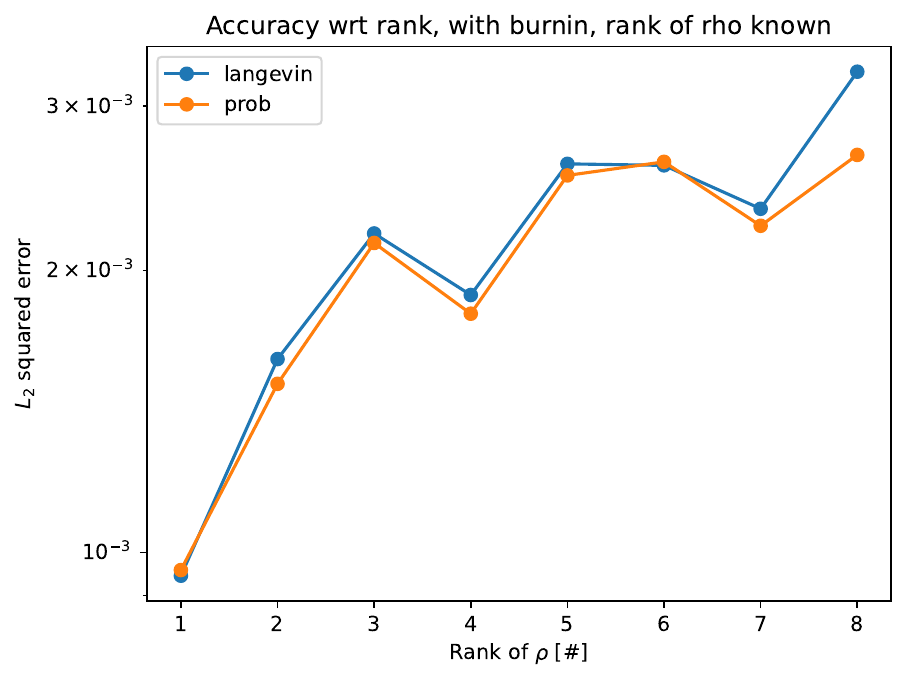
\includegraphics[width=\textwidth]{figures/experiments/rank_info/rank_known-1.png}
    
            \caption{Rank of $\rho$ known}
    
            \label{fig:rank-info-sub}
    
        \end{subfigure}
        \hfill
        \begin{subfigure}[b]{0.49\textwidth}
    
            % experiments/rank_not_known
    
            \centering
    
            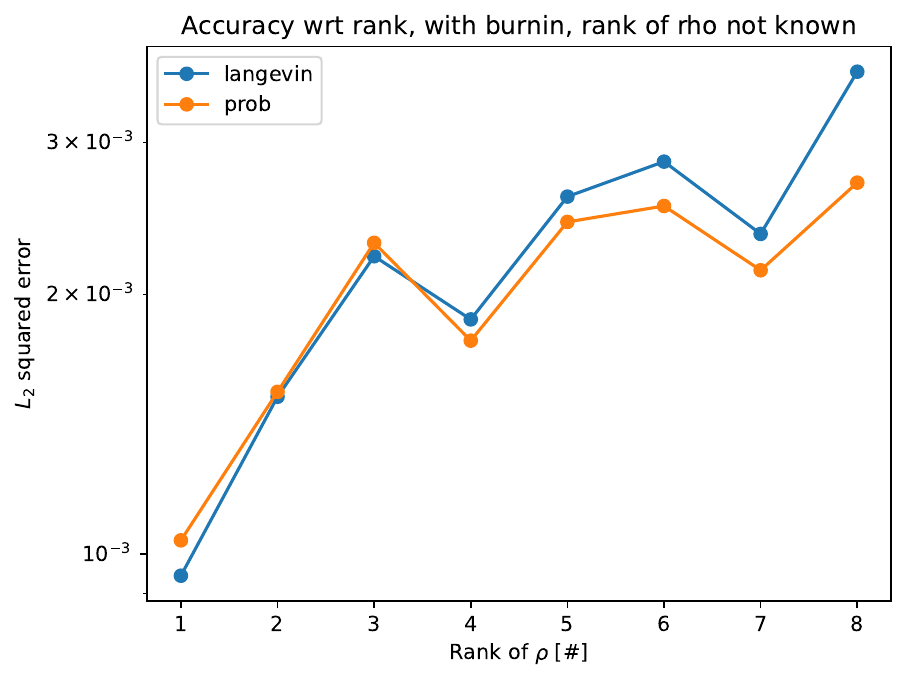
\includegraphics[width=\textwidth]{figures/experiments/rank_info/rank_not_known-1.png}
    
            \caption{Rank of $\rho$ not known}
    
            \label{fig:rank-no-info-sub}
    
        \end{subfigure}
        
        \label{fig:rank-info}
    
    \end{figure}
    $\Longrightarrow$ The information about the rank only marginally affects the accuracy
\end{frame}

\begin{frame}{Summary}
    \begin{itemize}
        \item Quantum tomography is not yet a solved problem, especially for large  systems
        \item MCMC methods are a promising direction of research, thanks to uncertainty quantification and prior information 
        \item The choice of the algorithm might have more impact on the convergence speed and accuracy than the prior
    \end{itemize}
    % - The Projected Langevin algorithm requires less iterations and is more accurate for larger $n$ than the prob-estimator, however it does not scale in terms of computation time
    % - Its convergence speed and accuracy are due to a combination of prior \textit{algorithm}, not just the prior
\end{frame}
\begin{frame}{Future work}
    \begin{itemize}
        \item Extend tests to larger $n$ to check for robustness of conclusions
        \item Try other gradient-based algorithms to see the impact on convergence speed (for example HMC)
        \item Try other priors to see the impact on computation time (the gradient may be faster to compute) and accuracy
    \end{itemize}
\end{frame}
\begin{frame}{References}
    \printbibliography
\end{frame}
\begin{frame}{Prob-estimator: full}
    It can be seen as eigendecomposition, without the orthogonality property:
    \begin{equation}
        \rho = U\Lambda U^\dagger
    \end{equation}
    Prior:
    \begin{equation}
        \pi(\rho) = \pi_1(\gamma_1, \dots, \gamma_d) \prod_{i=1}^d \pi_{2, i}(V_i)
    \end{equation}
    Likelihood:
    \begin{equation}
        \pi(\tb D| \rho) = \pi(\rho, \mb D) = \exp(-\lambda \ell(\rho,\mb D))
    \end{equation}
    with:
    \begin{equation}
        \ell(\rho, \mb D) = \sum_{\mb a \in \mathcal{E}^n} \sum_{\mb s \in \mathcal{R}^n} \left[\tr(\rho P^{\mb a}_{\mb s}) - \hat p_{\mb a,\mb s}\right]^2
    \end{equation}
    Posterior:
    \begin{equation}
        \pi(\nu|\tb D) \propto \exp(-\lambda\ell(\nu, \mb D)) \pi(\nu)
    \end{equation}
\end{frame}
\begin{frame}{Projected Langevin: full}
    Prior:
    \begin{equation}
        \nu_{\theta} (Y) = C_\theta \det(\theta^2I_d + YY^\dagger)^{-(2d+r+2)/2}
    \end{equation}
    Likelihood: 
    \begin{equation}
        L(Y, \mb D) = \sum^{M}_{i=1} (\hat p_m - \tr(A_mYY^\dagger))^2
    \end{equation}
    Posterior:
    \begin{equation}
        \hat \nu_{\lambda, \theta}(Y, \mb D) = \exp(-f_{\lambda, \theta}(Y, \mb D))
    \end{equation}
    with \begin{equation}
        f_{\lambda, \theta}(Y, \mb D) = \lambda \sum^{M}_{i=1} (\hat p_m - \tr(A_mYY^\dagger))^2 + \cfrac{2d + r + 2}{2}\log \det(\theta^2I_d + YY^\dagger)
    \end{equation} 

\end{frame}
\begin{frame}{Potential future experiments}
    \begin{itemize}
        \item Try experiemnts with more qubits to draw more robust conclusions
        \item Test with other algorithms and priors to see if its a property of this prior in particular, or it generalizes (The calculation of the graidient is going to be more costly in all cases)
        \item Try to use HMC to see if it still converges as fast for higher dimensions
    \end{itemize}
    
\end{frame}

\end{document}

